\section{Detailed Design}
\subsection{File System}

The file system at its core is responsible for storing encrypted user credentials in a secure manner. User credentials are passed (over USB) from the software client to the auxiliary MCU for encryption and storage on the internal EEPROM based file system. The design methodology adopted in this regard is to ensure that decryption of file system contents is only possible with a private key which is stored on the client side. \hyperref[sec:fsh]{Appendix B.1.1} and \hyperref[sec:fscpp]{Appendix B.1.2} are the C++ source code of the resulting file system implementation.
\subsubsection{Structure}

Figure 5.1 depicts the general structure of the file system. It is seen to consist of a header, global file table (GFT) and a series of file 'nodes'. The header field identifies the file system type and contains information on various parameters of the file system such as: total EEPROM size, node size, etc. The header field is written to during a formatting operation. A node is defined as a data structure that holds file data as well as a pointer to the next file block (node). The GFT is the entity which maps logical files to their corresponding node entries and contains information on a file such as it's name, size and offset to it's first node.
\begin{figure}[H]
\centering
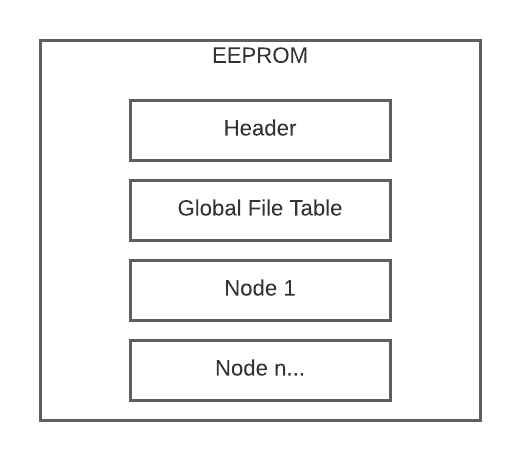
\includegraphics[width=0.4\columnwidth]{Figures/Fig_19.png}
\caption{File system structure.}
\label{fig:gantt}
\end{figure}

The file system does not support directories. It is also worth mentioning that the EEPROM space on the ATmega328P is limited to 1024B and therefore node sizes should be kept small (approx 128B each) in order to store a reasonable amount of credentials. In order to extend the maximum number of credentials an external EEPROM could be used. For 1024B, 24 bytes is allocated to the header and 70 bytes allocated to the global file table (GFT). Finally the remaining 930 bytes are allocated to file nodes. Since file nodes will be around 128 bytes the maximum number of credentials that can be stored is 7.

\subsubsection{Header}
Table 4 depicts the various fields of a header. The first field consists of the file system identifier, the 'magic id' which always retains a value of 0xABCD. This value identifies that the file system is of a compatible type. The second entry consists of the GFT (global file table) offset, this is a byte offset to the GFT structure from the beginning of the EEPROM. The total number of GFT entries is given by field 3. Since this value is a single byte the maximum number of entries can be 255. The fourth entry is the total EEPROM space available on the file system, this field is 2 bytes thus supporting file systems up to 64kB in size. 
\begin{table}[H]
\centering
\begin{tabular}{|r|l|}
\hline
\multicolumn{1}{|l|}{\textbf{Size (Bytes)}} &  \textbf{Description} \\ \hline
2 & Magic id. \\ \hline
1 & GFT offset.\\ \hline
1 & GFT entry count\\ \hline
2 & File system size. \\ \hline
1 & Node size.\\ \hline
1 & Node count. \\ \hline

\end{tabular}
\caption{File system header fields.}
\label{tbl:HWSWRequirements}
\end{table}

The fifth entry is a 1 byte field containing the size in bytes of a file system node, this can be up to 255 bytes in length. Finally the last field in Table 3 holds the total node count.
\subsubsection{Global File Table}

Table 5 details the fields for a single GFT entry. The first entry is a 1 byte boolean field which determines if the current GFT entry is in use. When this field is set to false and a new file created the corresponding GFT entry will be overwritten. The second entry consists of a 5 byte field holding the name of a file. Since one byte is used for the C style null terminator files can be up to four characters in length. Entry 3 in the GFT holds the total file size, this is a 2 byte field so file sizes up to 64 kB are supported. Finally the last field of Table 4 consists of a byte offset to the first node entry of the file.

The total size of the GFT structure is 10 bytes. Since 70 bytes have been dedicated to GFT's a total of 7 GFT's can be allocated by the filesystem. The search for an empty GFT entry is linear with each GFT index being probed for an inactive entry.

During a file read the corresponding node offset is retrieved and the node characteristics such as total size and utilization fetched. The contents of EEPROM for each node are then copied to memory to retrieve the file contents.
\begin{table}[H]
\centering
\begin{tabular}{|r|l|}
\hline
\multicolumn{1}{|l|}{\textbf{Size (Bytes)}} & \textbf{Description} \\ \hline
1 & Active. \\ \hline
5 & Filename. \\ \hline
2 & File size.\\ \hline
2 & First node offset.\\ \hline

\end{tabular}
\caption{GFT entry structure.}
\label{tbl:HWSWRequirements}
\end{table}



\subsubsection{Nodes}
Nodes have a similar structure to that of a linked list. Table 6 depicts their structure. The first field is a boolean field which determines if the current node is in use. The second field consists of a single byte representing the total utilization in bytes of a node, here it can be seen that a single node can hold up to 255 bytes. The second entry contains a pointer or byte offset to the next node of the file. If a value of 0xFFFF is specified for this field it will be assumed that this is the last node of the file. Finally the actual file data to be stored follows, n can be a maximum value of 255.

\begin{table}[H]
\centering
\begin{tabular}{|r|l|}
\hline
\multicolumn{1}{|l|}{\textbf{Size (Bytes)}} & \textbf{Description} \\ \hline
1 & Active. \\ \hline
1 & Node utilization. \\ \hline
2 & Next node offset.\\ \hline
n & file data (n bytes).\\ \hline

\end{tabular}
\caption{File system header fields.}
\label{tbl:HWSWRequirements}
\end{table}
\subsubsection{Public API}
This section details the various function prototypes as defined in the source code for for the filesystem (\hyperref[sec:fsh]{Appendix B.1.1} and \hyperref[sec:fscpp]{Appendix B.1.2}). Here the function prototypes that are exposed as public functions are described. In total the filesystem API exposes five main functions to handle file IO, these mainly relate to reading, writing and deleting files as well as reading and writing the filesystem headers.

\lstset{
numbersep=8pt, 
frame = single, 
language=C, breaklines,
%basicstyle=\footnotesize,%
showstringspaces=false,
columns=fullflexible,
literate = {-}{-}1
}


\textbf{Signature: } 
\begin{lstlisting}[language=C]
int format_fs()
\end{lstlisting}
\textbf{Description: }  \linebreak
Formats filesystem. EEPROM is first zero'd before writing the filesystem header.
\clearpage
\textbf{Signature: } 
\begin{lstlisting}[language=C]
struct fs_header read_fs_header()
\end{lstlisting}
\textbf{Description: }  \linebreak
Read filesystem header, return as \textbf{fs\_header} struct.

\textbf{Signature: } 
\begin{lstlisting}[language=C]
int write_file(struct fs_header *hd, char *name, char *data, int len)
\end{lstlisting}
\textbf{Description: }  \linebreak
Write \textbf{data} to filesystem specified by \textbf{hd}. The filename \textbf{name} should be specified as well as the data length. If a file already exists with the same name its data will be overwritten. The value returned will be the byte offset of the file's first data node in EEPROM storage.

\textbf{Signature: } 
\begin{lstlisting}[language=C]
char *read_file(struct fs_header *hd, char *filename, int *size)
\end{lstlisting}
\textbf{Description: }  \linebreak
Read file contents of file with \textbf{filename} on filesystem specified by \textbf{hd}. File contents will be returned as a character array/pointer. Additionally the total size in bytes of the file is written to the variable \textbf{size}.

\textbf{Signature: } 
\begin{lstlisting}[language=C]
int delete_file(struct fs_header *hd, char *filename);
\end{lstlisting}
\textbf{Description: }  \linebreak
Delete file with \textbf{filename} from filesystem \textbf{hd}.

\textbf{Signature: } 
\begin{lstlisting}[language=C]
struct fs_gft_entry *list_files(struct fs_header *hd, int *num)
\end{lstlisting}
\textbf{Description: }  \linebreak
List all files in filesystem specified by \textbf{hd}. Entries will be returned as a \textbf{fs\_gft\_entry} struct with a structure given by table 5. The total number of file entries is written to the variable \textbf{num}.

\subsection{Crypto Module}

The cryptography module is responsible for encrypting credentials sent from the software client and is located on the auxiliary microcontroller. It implements RSA encryption with a public exponent of 3 and a 1024 bit modulus. For RSA encryption the ciphertext may be obtained from the plain-text using the following formula:
\[ c = m^e\,mod\,n\]

It is worth noting that m and n are large integers and cannot fit in the standard \textbf{long int} C data type (4 bytes on Arduino). Therefore the implementation of RSA encryption requires the creation of an abstract class that can multiply and take the modulus of arbitrary large numbers. RSA-1024 encryption will be developed from the ground up without relying on OpenSSL. \hyperref[sec:rsah]{Appendix B.1.3} and \hyperref[sec:rsacpp]{Appendix B.1.4} are the C++ source code of the resulting cryptographic implementation. \hyperref[sec:eflow]{Appendix H} is a flow diagram for the resulting encryption/decryption steps.

\subsubsection{OpenSSL}
OpenSSL is the main cryptography library used for generating RSA keys and decrypting encrypted credentials parsed from the auxiliary MCU to the software client. It has a range of methods to perform both raw and padded RSA encryption/decryption. To generate a 1024 bit private key the following command can be issued:
\begin{lstlisting}[language=bash, frame=none]
$ openssl genrsa -3 -out rsa1024.pem 1024
\end{lstlisting}

This will generate an RSA key with a public exponent of 3 and save the result as a PEM or base64 encoded file. The various key parameters such as modulus, public and private exponent, etc may be extracted from a PEM file using the following command:
\begin{lstlisting}[language=bash, frame=none]
$ openssl rsa -in rsa1024.pem -text -inform PEM -noout
\end{lstlisting}

A C based OpenSSL API is also exposed and \textbf{RSA\_generate\_key()} can be called to create an RSA key of a specific bit length and public exponent. For decryption \textbf{RSA\_private\_decrypt()} can be called from C and supports raw and PKCS padded decryption/encryption. To extract the modulus from an RSA key first \textbf{PEM\_read\_RSAPrivateKey()} should be called to read the PEM formatted key followed by \textbf{RSA\_get0\_n()}.
\subsubsection{Number}

The \textbf{number} C class (defined in \hyperref[sec:rsacpp]{Appendix B.1.4}) is an abstraction that represents an arbitrary length number. It has the following structure:
\begin{lstlisting}[language=C]
typedef struct _number
{
  int id;
  int is_negative;
  int size_max;
  int size;
  unsigned char *bytes;
} number;
\end{lstlisting}

The \textbf{number} class is seen to consist of an \textbf{id}, which uniquely identifies each number as well as negation marker (\textbf{is\_negative}) to determine whether a number is negative or positive. Additionally a number has a maximum capacity (in bytes) \textbf{size\_max} as well as byte counter \textbf{size}. Finally the class contains a pointer to an array of bytes representing the number (\textbf{bytes}).

The crypto module implements a number of internal functions to multiply and take the modulus of two arbitrary length numbers (\hyperref[sec:rsacpp]{Appendix B.1.4}):

\textbf{Signature: } 
\begin{lstlisting}[language=C]
void number_multiply(number *x, number *y, number *output)
\end{lstlisting}
\textbf{Description: }  \linebreak
Multiplies  two arbitrary length numbers \textbf{x} and \textbf{y} together and stores result in \textbf{output}.

\textbf{Signature: } 
\begin{lstlisting}[language=C]
void number_modulus(number *x, number *y)
\end{lstlisting}
\textbf{Description: }  \linebreak
Calculate \textbf{x} \% (mod) \textbf{y} of two arbitrary length numbers and stores result into \textbf{x}.

\textbf{Signature: } 
\begin{lstlisting}[language=C]
number *number_pow3m(number *x, number *n)
\end{lstlisting}
\textbf{Description: }  \linebreak
Calculates the corresponding ciphertext c for e=3:\[ c = x^3\,mod\,n\]
In order to raise x to the power of 3 the number x would have to be multiplied by itself 3 times. However since x is large the resulting number would take up a large amount of memory. For memory efficiency and performance it is better to break up the modulus into two parts. The algorithm used to perform this task is based on the following identity:
\[ x^3\,mod\,n = x(x^2\,mod\,n)\,mod\,n\]

The output returned is a pointer to the resulting \textbf{number}.
\subsubsection{RNG}
The RNG (Random Number Generator) used for generating the random bytes for PKCS padding is important and ensures that the output ciphertext is different each time for the same input plain-text. RSA encryption without padding is deemed insecure. In order to generate random numbers two approaches are possible. The first involves the use of the standard library \textbf{stdlib.h}, specifically \textbf{rand()} and \textbf{srand()}. 

\textbf{rand()} generates a pseudo random number from 0 to \textbf{RAND\_MAX}(32767) while \textbf{srand()} sets the seed value for the RNG. A common seed to use for \textbf{srand()} is the current system time, another possibility is to use to voltage of a floating pin of a microcontroller which is also a pseudo random process.

Another approach is to use Arduino's built in \textbf{random()} and \textbf{randomseed()} functions which are similar in operation to the standard library versions.
\subsubsection{PKCS\#1 Padding}
RSA encryption is a deterministic process, that is, it has no random component. As a result it is susceptible to a range of cryptanalytic attacks. For example one approach to cracking a ciphertext is to simply encrypt a range of plain-text pairs with the public key and compare it to the corresponding ciphertext for a match. 

Therefore some form of randomness should be present in the message string being encrypted and this is the goal of RSA padding schemes. PKCS \#1 (Public Key Cryptography Standards) is a family of standards published by RSA Laboratories. It provides recommendations for implementing RSA for public key cryptography. PKCS\#1 v1.5 is an encryption padding scheme defined by the standard. It is also supported by OpenSSL. 
The standard specifies that a plain-text block to be encrypted (x) should be formatted as follows:
\begin{lstlisting}[language=bash, frame=none]
x = 0x00 || 0x02 || r || 0x00 || m
\end{lstlisting}

Here r represents a series of random numbers and m the original message. The minimum length of x should be 11 bytes in total. Additionally the minimum length of r should be 8 bytes. The encryption algorithm then becomes:

\[ c = x^e\,mod\,n\]

\subsubsection{Public API}



\textbf{Signature: } 
\begin{lstlisting}[language=C]
void number_rsa_pkcs(unsigned char *str,
                     int size,
                     unsigned char *modulus,
                     unsigned char *output,
                     int rsa_bits);
\end{lstlisting}
\textbf{Description: }  \linebreak
Given a plaintext string \textbf{str} of length \textbf{size}, encrypt \textbf{str} using the specified \textbf{modulus} and a public exponent e=3. The number of rsa key bits is specified by \textbf{rsa\_bits}. The resulting ciphertext is stored in \textbf{output}. The padding scheme used is PKCS\#1 v1.5.


\subsection{USB Driver}

\subsubsection{Schematic}
Figure D.1 (\hyperref[sec:appd1]{Appendix D}) depicts the schematic for the USB driver portion of the overall system. It is seen to consist of a 16MHz crystal oscillator connected to input ports PB6 and PB7 supported by two 22pF load capacitors C1, C2. Additionally ports PD2 and PD3 connect directly to the D+ and D- pins of a USB adapter. Resistors R1 and R2 serve to limit the total current through each data wire. Finally R3 serves as a pull up resistor to set the transient state of data pin D-.

RX(serial) port PD0 then connect to the corresponding TX port of the auxiliary MCU while TX port PD1 connects to the RX port of the auxiliary MCU. It should be noted that VCC should be a 3.3V source in order to conform to USB 1.1 specifications for logic levels. Microcontroller U1 forms the second part of the overall system circuitry besides the auxiliary MCU.

\hyperref[sec:usbmcu]{Appendix B.2} are the corresponding C sources for the USB driver implementation.

\subsubsection{USB 1.1}
Universal serial bus (USB) is an industry standard specification for the communication between hardware peripherals and computers. Currently four generations of USB exist, namely USB 1,2,3 and most recently USB 4. For backwards compatibility reasons USB 1.1 was chosen allowing for the use of the standard male/female USB cabling rather than new adapter types such as USB-C.

A USB system consists of a USB host followed by multiple communication pipes to various logical entities termed endpoints (Figure 5.2). An endpoint corresponds to a data buffer and can be categorized into either a control or data endpoint.

\begin{figure}[H]
\centering
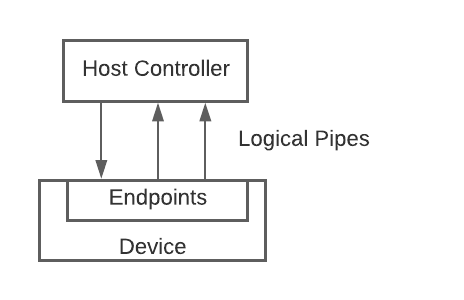
\includegraphics[width=0.4\columnwidth]{Figures/Fig_68.png}
\caption{USB system summary.}
\label{fig:gantt}
\end{figure}

Here the host controller is typically a computer while the device is usually some embedded system or micro-controller such as U1 in Figure D.1 (\hyperref[sec:usbmcu]{Appendix D}). Control endpoints are typically bidirectional and are used to configure the device, obtain device information or perform control actions relevant to the device. Data endpoints are used for transferring data in and out from the host controller, this may include information such as serial data. In USB the direction of an endpoint may be IN or OUT and is relative to the host. Therefore IN refers to transfers to the host from the device and OUT always refers to transfers from the host to the device \cite{usb_endpoints}.

For our use case we wish to transport serial data in a bidirectional manner between the host (PC) and device (USB driver MCU) and therefore a variety of endpoints are required to achieve this. Various classes of USB device exist however this paper will focus on emulating low speed USB functionality for the communication device class using an open source AVR USB stack known as V-USB.

\subsubsection{V-USB}
V-USB is a software only USB stack which provides low speed USB interfacing for AVR based microcontrollers. The ATmega328 microcontroller which is used for both the auxiliary MCU and USB driver MCU does not have native hardware support for USB and therefore a software implementation of USB is required. V-USB supports one control endpoint, two interrupt/bulk-in endpoints and up to 7 interrupt/bulk-out endpoints making it more than sufficient for transporting serial data.

It requires an AVR microcontroller with at least 2kB of flash memory , 128 bytes of RAM and a clock rate of at least 12MHz. All high level functionality is written in C and the code is well documented.

\subsubsection{CDC ACM}
The communication device class allow USB devices to emulate legacy serial ports. Before USB was fully standardized most interfacing to hardware (i.e floppy disks and printers) was done through RS232 ports. RS232 is a telecommunications standard that was adopted for the transmission of serial data. When USB was standardized it became apparent that emulation of older RS232 technologies was required. ACM (abstract control model) is a subclass of CDC that describes a bidirectional communication flow known as a virtual serial port. 

Specifically ACM contains two interfaces termed COMM and DATA. The COMM interface contains one IN endpoint and is used to notify the host about the current serial state while the DATA interface contains one IN and one OUT bulk endpoint. The data interface allows the host to send and receive bulk serial data.

One advantage of the CDC ACM class is that no specific drivers are required for interfacing when using an operating system based on the Linux kernel. In fact devices conforming to the CDC ACM class appear in \textbf{/dev/} as \textbf{ttyACM*} (i.e a virtual serial port) where * represents a number from 0 and above. The list of available ACM devices on a Linux host may be queried using the following command:

\begin{lstlisting}[language=bash, frame=none]
ls /dev/ | grep ttyACM
\end{lstlisting}

\subsubsection{Internal API}

A description of the various function prototypes is derived from the source in \hyperref[sec:usbmcu]{Appendix B.2}. Additionally the control flow for the driver is shown in Figure G.1 (\hyperref[sec:usbflow]{Appendix G}).

\textbf{Signature: } 
\begin{lstlisting}[language=C]
unsigned char usbFunctionDescriptor(usbRequest_t *request)
\end{lstlisting}
\textbf{Description: }  \linebreak
Return USB descriptor upon request. The required descriptor is defined by the global variable \textbf{usb\_descriptor}. This defines a CDC ACM device as well as the various endpoints required by the class.

\textbf{Signature: } 
\begin{lstlisting}[language=C]
unsigned char usbFunctionSetup(unsigned char *bytes)
\end{lstlisting}
\textbf{Description: }  \linebreak
Handle USB setup.


\textbf{Signature: } 
\begin{lstlisting}[language=C]
unsigned char usbFunctionRead(unsigned char *data, unsigned char len)
\end{lstlisting}
\textbf{Description: }  \linebreak
Transfer block of data from driver MCU to host computer via USB. Transfers serial data ready to be sent to host computer.


\textbf{Signature: } 
\begin{lstlisting}[language=C]
unsigned char usbFunctionWrite(unsigned char *data, unsigned char len)
\end{lstlisting}
\textbf{Description: }  \linebreak
Store block of data sent from host computer to driver MCU via USB.

\textbf{Signature: } 
\begin{lstlisting}[language=C]
void iuart(unsigned char db, //databits,
           unsigned char dp, // parity,
           unsigned char sb, // stop bit,
           unsigned long tx_rate); // transfer rate);
\end{lstlisting}
\textbf{Description: }  \linebreak
Initialize UART on driver MCU with the specified baud rate \textbf{tx\_rate}

\textbf{Signature: } 
\begin{lstlisting}[language=C]
void puart();
\end{lstlisting}
\textbf{Description: }  \linebreak
Poll driver MCU for serial data ready to be sent or received from UART buffer. If serial data is received from the RX line (port PD0) this data is forwarded to usbFunctionRead. If USB data is transferred from the host computer via the virtual serial port to the driver MCU (usbFunctionWrite) it is transmitted on the UART TX port (PD1).

\subsection{Communication Logic}
Communication between the software client and auxiliary MCU is essential to the operation of the overall system. Some form of message formatting is required if these two endpoints are to communicate with one another. Additionally a list of commands supported by the auxiliary MCU should expose functionality of both the file system and crypto module.

The formatting adopted for commands is shown below:
\begin{lstlisting}[language=bash, frame=none]
$command$param_1$param_n$
\end{lstlisting}

This string is required to be sent over the virtual serial port from the software client to the USB driver MCU. The USB driver MCU then forwards the corresponding serial command data to the auxiliary MCU which performs command processing as well as the corresponding file and cryptographic related operations.

\subsubsection{Serial Commands}
Serial communication was chosen as it is relatively straightforward to implement and due to the fact that it is supported natively in hardware on the ATmega328 microcontroller through the integrated UART transceiver. It is also supported by the Arduino software core which provides serial functionality through the \textbf{Serial} class. In order to issue the following commands manually a serial terminal must be connected to the driver MCU using a program such as the Arduino serial monitor \cite{serial_monitor}.

\textbf{Signature: } 
\begin{lstlisting}[language=bash]
$encrypt$modulus$data$filename$
\end{lstlisting}
\textbf{Description: }  \linebreak
Encrypts \textbf{data} using RSA-1024 with the specified \textbf{modulus} and stores the result on the filesystem under the name \textbf{filename}. The modulus must be specified as a hexadecimal string of 256 characters in length. The filename is limited to four characters in length. The modulus of the master PEM file can be retrieved in hexadecimal form using the following command:
\begin{lstlisting}[language=bash, frame=none]
openssl rsa -in rsa1024.pem -noout -modulus | sed 's/Modulus=//'
\end{lstlisting}

\textbf{Signature: } 
\begin{lstlisting}[language=bash]
$list$
\end{lstlisting}
\textbf{Description: }  \linebreak
Retrieves the filename of all files stored on filesystem.

\textbf{Signature: } 
\begin{lstlisting}[language=bash]
$read$filename$
\end{lstlisting}
\textbf{Description: }  \linebreak
Read contents of \textbf{filename} and return as hexadecimal string.

\textbf{Signature: } 
\begin{lstlisting}[language=bash]
$delete$filename$
\end{lstlisting}
\textbf{Description: }  \linebreak
Deletes file with \textbf{filename} from the master filesystem.

\textbf{Signature: } 
\begin{lstlisting}[language=bash]
$format$
\end{lstlisting}
\textbf{Description: }  \linebreak
Remove all files and format filesystem.

\textbf{Signature: } 
\begin{lstlisting}[language=bash]
$help$
\end{lstlisting}
\textbf{Description: }  \linebreak
Display help prompt with a list of available commands.

Each command issued over the serial port will either return an OK status or FAIL status depending on the parameters provided.

\subsubsection{Auxiliary MCU}

Figure D.2 (\hyperref[sec:appd2]{Appendix D}) depicts the circuit diagram of the auxiliary MCU that handles serial communication and processes each serial command respectively. It is seen to consist of a 16MHz crystal and two 22pF load capacitors C1, C2. Additionally the RX line (PD0) of the auxiliary MCU is connected to the TO\_RX net of the USB driver MCU and the TX line (PD1) is connected to the TO\_TX net of the USB driver MCU. These connections ensure that serial communication flows from the host computer through the USB driver to the auxiliary MCU and vice versa. \hyperref[sec:comm]{Appendix B.1.5} is the source code for the main entry point of the auxiliary MCU.

The implementation of command processing at the auxiliary endpoint firstly relies on the allocation of a 400 byte data buffer. 400 bytes accounts for a 256 byte modulus (represented as a hexadecimal string), 100 bytes for the password length and reserve bytes for the filename and command string. A call to \textbf{Serial.readBytes} is then made to read a block of serial data to the buffer:

\begin{lstlisting}[language=C]
buffer = malloc(400);
Serial.readBytes(buffer, 400);
\end{lstlisting}

The command string is then extracted from the buffer using the \textbf{strtok} C library method which breaks up a string into a series of tokens given a delimiter character.
\begin{lstlisting}[language=C]
char *cmd = strtok(buffer, "$");
\end{lstlisting}

Finally the \textbf{cmd} buffer is compared against known command strings using \textbf{strcmp} and a variable called \textbf{pid} set to a numerical value corresponding to a command.

\begin{lstlisting}[language=C]
 if(strcmp_P(cmd, (PGM_P)F("help")) == 0){
          pid = 7;
    }
\end{lstlisting}

Then further down the main loop the command corresponding to a particular \textbf{pid} is executed and any additional command parameters extracted with further calls to \textbf{strtok}. Due to the limited dynamic memory of the ATmega328P and the overhead associated with RSA encryption careful management of memory is required in order to prevent memory leaks which eventually lead to memory exhaustion and MCU lockup.


\subsection{Software Client}
At the client end communication is required to poll the state of the filesystem and issue commands to encrypt data. Additionally some form of communication with the client browser extension would be required. The choice of browser support was based on browser usage statistics from \cite{browser_stats} which indicates that chrome currently has 64\% of the browser market share. Therefore chrome is the selected target platform for developing a browser extension.

Google chrome provides communication with external C/C++ programs through its native messaging API \cite{native_messaging}. C/C++ programs register as 'messaging hosts' through a metafile written to a specific directory. For Google Chrome on Linux this directory is shown below: 

\begin{lstlisting}[language=bash, frame=none]
~/.config/google-chrome/NativeMessagingHosts/
\end{lstlisting}

The meta-file is a JSON file which contains the name of the native host along with a path to the executable file to communicate with. Communication is through the standard input and output streams and a C based library exists known as \textbf{libnativemsg} to parse messages from Google Chrome as well as send native messages \cite{lib_native}. With the ability to communicate with a browser extension the remaining tasks include opening a serial connection to the USB driver MCU as well as parsing messages between the native host and browser extension. 

It is worth mentioning that communication with native hosts involves the transport of JSON formatted text. Therefore a JSON parsing library written in C was required and \textbf{cJSON} was chosen for this purpose \cite{c_json}. Finally a C/C++ library providing support for serial communication was required and a cross platform library known as \textbf{seriallib} was chosen \cite{serial_lib}.

The software client is responsible for generating and storing cryptographic keys as well as RSA decryption. The flow of credential information in the overall system should work as follows: the user types in their username and password on a web form, the credential is then captured and an encryption request sent over serial with the modulus of the PEM key that is stored in a users home folder. The resulting credential is then encrypted using RSA-1024 encryption and stored on the auxiliary microcontrollers EEPROM. When the users visits the same login portal a request to the file system is made and the corresponding encrypted credential read from the filesystem and decrypted using the master PEM file. The username and password fields are then automatically filled in and an authentication request submitted using the browser extension's JavaScript submission engine.
\subsubsection{Native host}
Communication with the browser extension, to provide facilities to query the filesystem and perform encryption/decryption, is accomplished through the native messaging host. The native host acts as a middle man between the auxiliary microcontroller and browser extension. The source code for the native host is shown in \hyperref[sec:mainc]{Appendix C.1.1}.

The first task of the native host is to establish a serial connection with the USB driver microcontroller. This is accomplished with the following code:
\begin{lstlisting}[language=C]
char buffer[400];
// ...
command = popen("ls /dev/ | grep ttyACM", "r");
if(fgets(buffer, sizeof(buffer), command) ==NULL){
    exit(EXIT_FAILURE);
}
strtok(buffer,"\n");
sprintf(temp, "/dev/%s", buffer);
code = serial.openDevice(temp, 115200);
\end{lstlisting}

First a list of ACM devices is queried using \textbf{popen}, the result of the command is then written to \textbf{buffer} and the corresponding newline character stripped. Next a call to \textbf{serial.openDevice} is made (\textbf{serialib}) with the specified baud rate of 115200 bits per second. Native messages passed from the browser to the native host are captured using the following code:
\begin{lstlisting}[language=C]
uint8_t *msg = NULL;
// ...
msg = nativemsg_read(&len);
\end{lstlisting}

The resulting text stored in \textbf{msg} is a JSON string and must be parsed with cJSON:
\begin{lstlisting}[language=C]
cJSON *json = NULL;
cJSON *cmd = NULL;
// ...
json = cJSON_Parse(msg);
cmd = cJSON_GetObjectItem(json, "cmd");
    
if (cmd)
{
    if (strcmp(cmd->valuestring, "delete") == 0)
    {
        exec_delete(&serial, buffer, filename);
// ...
\end{lstlisting}
The command strings are then matched using \textbf{strcmp}. If the conditional statement evaluates to true then the browser extension has requested a command and the appropriate serial command must be forwarded over the virtual serial port. For the case of the delete command a call to \textbf{exec\_delete} is made, this function is defined as follows:
\begin{lstlisting}[language=C]
int exec_delete(serialib *serial, char *buffer, char *filename)
{
    int count = 0;
    char local;
    serial->flushReceiver();
    sprintf(buffer, "$delete$%s$", filename);
    serial->writeString(buffer);
    int ret = probe_serial(serial, buffer);

    return ret;
}

\end{lstlisting}

First the serial receiver buffer is flushed (cleared) through a call to \textbf{serial.flushReceiver}. This sets the transient state of the serial port to idle. Next the serial command is formatted through a call to \textbf{sprintf} in the format defined in section 5.4.1. Then a call to \textbf{serial.writeString} is made to write the corresponding command and its arguments to the serial port which is then transferred to the driver MCU and subsequently relayed to and processed on the auxiliary MCU - with the results of the command being outputted once again to the serial port. A call to \textbf{probe\_serial} is made to retrieve the results of a command after they have been outputted by the auxiliary MCU. 
\subsubsection{Key Generation}
The generation of cryptographic keys is important in order to enable the encryption and decryption of password credentials. The maintenance of cryptographic keys is once again handled by the native host. RSA Key generation relies on OpenSSL. Specifically the following code block is applicable:
\begin{lstlisting}[language=C]
sprintf(buffer, "%s/%s", getenv("HOME"), "key.pem");
// Check for master key PEM
// If it doesn't exist create key
if (access(buffer, F_OK) != 0)
{
    // Open file for write operation
    FILE *fp = fopen(buffer, "w+");
    // Generate 1024 bit key, e=3
    rsa = RSA_generate_key(1024, 3, 0, 0);
    // Write PEM
    PEM_write_RSAPrivateKey(fp, rsa, 0, 0, 0, 0, 0);
    fclose(fp);
}

\end{lstlisting}

This code block checks if a file called \textbf{key.pem} exists in the users home directory, if not calls to \textbf{RSA\_generate\_key} are made with parameters specifying a 1024 bit key length and a public exponent of 3. Finally the resulting PEM file is written with a call to \textbf{PEM\_write\_RSAPrivateKey}
\subsubsection{Decryption}
The decryption functionality is also handled by OpenSSL. Specifically the OpenSSL function \textbf{RSA\_private\_decrypt} is used to decrypt a 128 byte block of encrypted data using PKCS\#1 padding:
\begin{lstlisting}[language=C]
RSA_private_decrypt(128, buffer, temp, rsa, RSA_PKCS1_PADDING);
\end{lstlisting}

\subsubsection{Browser Extension}

Google chrome browser extensions, at minimum, consist of a \textbf{manifest.json} file together with a HTML template and background script. The source code for the browser extension is shown in \hyperref[sec:browser11]{Appendix C.2}. The \textbf{manifest.json} file used in the SecurePass extension is shown below:
\begin{lstlisting}[]

 {
  "name": "SecurePass Extension",
  "version": "1.0",
  "manifest_version": 2,
    "permissions": [
    "nativeMessaging",
    "webNavigation", 
    "*://*/*" ,
    "activeTab",
    "storage",
    "tabs"
  ],
  "browser_action" :{
    "default_popup" : "layout.html",
    "default_title" : "SecurePass"
  },
  "background": {
    "scripts": ["background.js"]
  }
}
\end{lstlisting}

It is seen to consist of a range of permissions to allow the extension to access native host messaging functionality, local storage as well as the active tabs context to extract specific DOM content and inject JavaScript code.

The background script \textbf{background.js} (\hyperref[sec:back]{Appendix C.2.1}) runs once per google chrome instance and is responsible for dispatching native messages to the native host which have been requested by the browser popup \textbf{layout.html}. \textbf{layout.html} defines the user interface of the extension in HTML and contains references to JavaScript logic to handle button input, communication with the \textbf{background.js} script as well as HTML rendering.

Within \textbf{background.js} a call to \textbf{connectNative} is made:
\begin{lstlisting}[]
var native = chrome.runtime.connectNative('com.secure.pass');
\end{lstlisting}

This spawns an instance of the native host and sets up the standard input and output streams to forward and receive JSON messages. The parameter passed to the the function is the name of the native host as defined in the native host's metadata file.

A communication port (listener) with the extension popup script (\textbf{script.js}) is opened using the following line of code:

\begin{lstlisting}[]
var port = 0;
// ...
chrome.extension.onConnect.addListener(function (lport) {
  port = lport;
  // ...
\end{lstlisting}

The \textbf{addListener} handler is called within \textbf{background.js} whenever a call to \textbf{postMessage} is made from the extension popup. Within the \textbf{addListener} handler a check for various message strings is made: 
\begin{lstlisting}[]
 // ...
 if (match == "list") {
    cmd = "list";
    native.postMessage({ cmd: "list" });
    console.log("posted message");
  }
 // ...
\end{lstlisting}

In the code snippet shown above a check for the \textbf{list} command is made. If the conditional statement evaluates to true then the global variable \textbf{cmd} is set to the command string. Finally a call to \textbf{native.postMessage} is made which sends the JSON key \textbf{cmd} and value \textbf{"list"} to the native host. The native host then processes the respective command and then writes back the result using \textbf{nativemsg\_write}. This result is then captured using the following handler (defined in \textbf{background.js}):

\begin{lstlisting}[]
native.onMessage.addListener(function (res) {
// ...
\end{lstlisting}

Finally the \textbf{cmd} parameter, within the handler, set earlier is compared and the results from the native host forwarded to the extension popup using \textbf{port.postMessage} where the corresponding data returned can be processed:

\begin{lstlisting}[]
// ...
if (cmd == "delete") {
    port.postMessage("[delete]" + res.msg);
}
// ...
\end{lstlisting}

Figure 5.5 shows the resulting user interface of the browser extension. It is seen to consist of a list of files on the EEPROM filesystem, together with input buttons to store a password and format the filesystem. Additionally buttons to decrypt a specific filesystem entry and display it as well as delete a filesystem entry are also present.

To use the browser extension first the user visits the corresponding web login portal, fills in their username and password and then clicks on the 'store password' button. An activity indicator will then show up until the encryption process is complete and the file stored on the filesystem. Then when the user visits the same login portal again the filesystem entry corresponding to the current login page will turn green and the password will automatically be decrypted and filled in.

\begin{figure}[H]
\centering
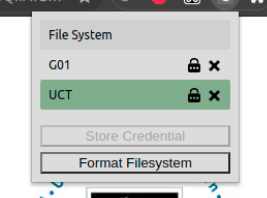
\includegraphics[width=0.35\columnwidth]{Figures/Fig_53.png}
\caption{User interface of browser extension.}
\label{fig:gantt}
\end{figure}

\subsubsection{SSO Capability}

SSO capability is provided through the browser extension described in section 5.5.4. When a google chrome instance is first launched the user is prompted for the master authentication key (\hyperref[sec:bext1]{Appendix I.1}). Once the user is authenticated and the browser extension clicked they will be presented the user interface shown in Figure 5.3. The user can then navigate to an online account portal, fill in the relevant login details and click 'Store Credential' (Figure F.1, \hyperref[sec:credflow]{Appendix F} for control flow). Next when the same login portal is visited again the login details will automatically be filled in and and the submission engine (JavaScript code that submits the login form) will take over and log the user in.

A video demonstration of the SSO system is shown in \hyperref[sec:SystemOverview]{Appendix A}

\begin{figure}[H]
\centering
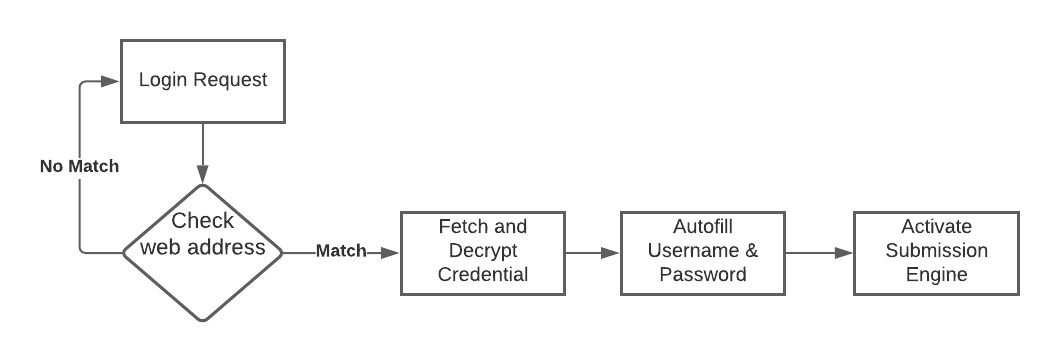
\includegraphics[width=0.9\columnwidth]{Figures/Fig_54.png}
\caption{SSO control flow.}
\label{fig:gantt}
\end{figure}

Figure 5.4 shows the general control flow of an SSO login request. Firstly the web address of the login portal is compared against a list of key, value pairs where the key is the root URL of the login portal and the value is the filename of the credential stored on the auxiliary MCU. If a key match is found then the relevant credential is fetched and decrypted. Next the username and password are extracted from the decrypted credential and the relevant fields on the login page automatically filled in. Finally the submission engine takes effect and the login request is submitted. The credential filename corresponding to a particular login portal will be highlighted green (Figure 5.3).

The user interface of the browser extension shown in Figure 5.3 allows an end user to store a credential pair when the user has entered the login credentials for a particular service portal. The method of credential extraction involves injecting JavaScript code that contains the following line:
\begin{lstlisting}[language=Java]
var elements = document.getElementsByTagName("input");
\end{lstlisting}

This line of JavaScript can be found within the \textbf{extractPassword} function of \textbf{script.js}.
\textbf{elements} then contains the required username and password fields which must be filtered according to the element type:
\begin{lstlisting}[language=Java]
 for (element in elements) {
            if (elements[element].type == "password" && ...) {
                password = elements[element].value;
            }
            if(elements[element].type == "email" | 
               elements[element].type == "text"){
              ... 
              
\end{lstlisting}

HTML password fields typically have the type set as "password" while username fields typically have a type of  "email" or "text". The required JavaScript is injected into the currently active tab using \textbf{chrome.tabs.executeScript}:

\begin{lstlisting}[language=Java]
chrome.tabs.executeScript({
            code: '(' + extractPassword + ')();'
        }, (results) => {
        ...
\end{lstlisting}


As shown in Figure 5.4 SSO capability is composed of a credential form auto filler as well as a submission engine. Credential auto-fill is accomplished through injecting JavaScript to set the HTML username and password elements within the variable \textbf{elements}. 

The submission engine's responsibility is to simulate a user pressing the 'Sign In' button on a log in portal. Due to to the wide variety of different HTML buttons, a variety of techniques are required in order to locate the correct button (Figure 5.5). This involves finding all HTML elements with an \textbf{'onclick'} attribute as well as \textbf{'button'} tags. Another possibility are inputs of type \textbf{submit}. Similar to credential extraction all code injection takes place using \textbf{chrome.tabs.executeScript}. 

The variable \textbf{code} within \textbf{background.js} (\hyperref[sec:back]{Appendix C.2.1}) contains the JavaScript to be injected for the submission engine.

\begin{figure}[H]
\centering
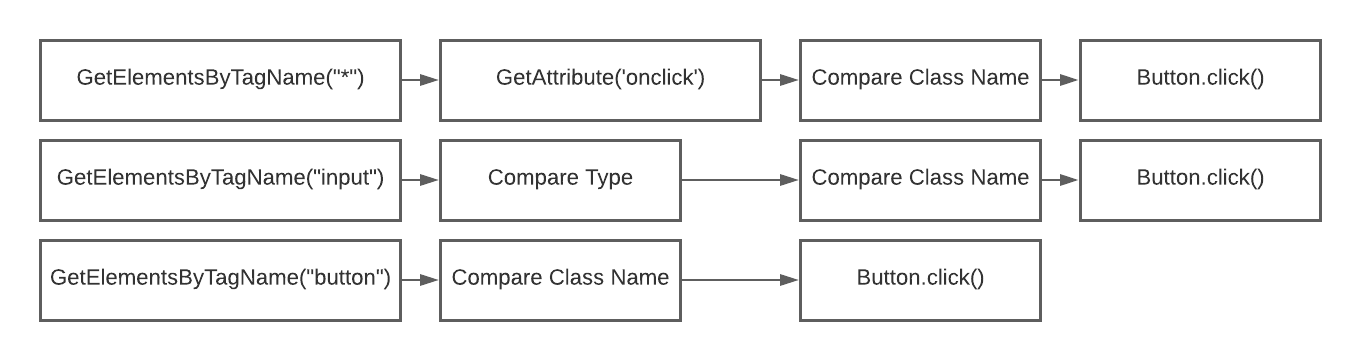
\includegraphics[width=1.1\columnwidth]{Figures/Fig_62.png}
\caption{Submission engine attempts to identify the login button.}
\label{fig:gantt}
\end{figure}

When a user selects 'Store Credential' within the browser extension UI the full URL of the active tab is fetched and the sub URL extracted (part of the URL without parameters). Next a key, value pair is created within local storage with the key being the sub URL and the value the filename of the credential stored on disk:

\begin{lstlisting}[language=Java]
chrome.storage.local.set({ [url]: filename }, function () {
        ...
\end{lstlisting}

Since the goal of the submission engine was to simulate a user clicking on the 'Log In' button the submission engine was tested against a variety of popular online services in order to ensure that SSO functionality was working correctly. The tests consisted of visiting the respective login portal of an online service, filling in the corresponding login details and then storing the credential using the browser extension UI. Then when the login page was revisited the credential auto-fill and submission engine functionality were tested to ensure the user was logged-in successfully. Results for these tests are shown in Table 7.

\begin{table}[H]
\centering
\begin{tabular}{|l|l|l|l|}
\hline
Test ID & Service            & Credential Autofill & Submission Engine \\ \hline
1       & Microsoft Outlook  & Pass                & Pass              \\ \hline
2       & Google Gmail       & Pass                & Pass              \\ \hline
3       & FNB Online Banking & Pass                & Pass              \\ \hline
4       & MyUCT Login        & Pass                & Pass              \\ \hline
5       & Instagram          & Pass                & Pass              \\ \hline
\end{tabular}
\caption{Credential autofill and submission engine tests.}
\end{table}


It should be noted that although the current SSO scheme works across a wide range of services, it is probable that the correct login button on a form with varying HTML styling might not be correctly identified in certain instances. This is one limitation to the pseudo SSO functionality of the current system. A more intelligent SSO client might involve the use of AI to identify HTML login elements more effectively.